\documentclass[journal]{IEEEtran}
\usepackage{blindtext}
\usepackage{graphicx}
\usepackage{siunitx}
\renewcommand{\vec}[1]{\mathbf{#1}}
\usepackage{float}
\usepackage{tabularx}
\ifCLASSINFOpdf

\else
 
\fi

\hyphenation{op-tical net-works semi-conduc-tor}


\begin{document}
\title{Astronomical Image Processing}
\author{D.Kololgi,~{Imperial College London}}

\maketitle

\section*{COVID-19 pandemic April 2020}
* This report was written after completing two of three weeks of lab 
access due to the teaching laboratory shutdown.

* This work was submitted before feedback from my Cycle 2 report was 
received.

* Demonstrators were unavailable in 2 / 8 scheduled lab sessions as a 
result of strike action. \newline

\begin{abstract}
This paper presents galaxy number counts in the SDSS r band filter over a range $7\,\leq\,m\,\leq\,20$ of magnitudes. The method involved reading a deep optical CCD image into a python IDE and using modularised coding to automatically catalogue galactic sources in the image. The main data set produced a sample size of $2181$ galaxies including poisson errors for the number counts and systematic instrument errors for the magnitudes. Between magnitudes $12\,\leq\,m\,\leq\,18$ there is a strong linear relationship with a gradient of $0.314\,\pm\,2.23\,\times\,10^{-4}$ in strong disagreement with the theoretical predictions from a homogeneous, isotropic galaxy distribution with fixed galactic luminosity. We further compare with external sources such as galaxy number counts by Yasuda et al. that illustrate a low sample-size effect present in this investigation. 
 
\end{abstract}

\section{Introduction}
The aim of this investigation was to use a deep optical CCD image of the extra-galactic sky to determine the relationship between source counts (galaxies in this case) and apparent magnitude values [1]. The motivation behind finding this relationship arises from the desire to test the Euclidean or non-Euclidean nature of the space-time geometry of the local universe. Using basic assumptions of a Euclidean (flat) space-time we derive, in the theory section, an expected relationship between number of sources to a given flux limit and their apparent magnitudes. If real data adhered to this then it could be seen as evidence that the local universe is or is close to being Euclidean in nature [2]. Measuring cosmological parameters, however, was not the main focus, rather this investigation involved developing a method to automatically detect and catalogue galaxies in a deep field image and then find a relationship between the counts and their apparent magnitudes on the AB magnitude scale. A core component of this meant determining when a galaxy ends and the background noise begins. Whatever method used to make this determination will be an approximate since the flux distribution of real galaxies are continuous, nonetheless, a measurement of the local background flux as a function of aperture area was made and if change in flux from a galaxy fell between $1\sigma$ away from the background mean it would signal the effective end of the galaxy. This method is a variable aperture technique that more precisely captures the true flux of the galaxy than simply having a fixed size aperture of a galaxy.
\section{Theory}
We begin a heuristic derivation [3] of the expected source counts brighter than a given magnitude limit by stating three assumptions. (1) Galaxies are uniformly distributed in space. (2) They all have the same luminosity. (3) The universe is of the Minkowski type (euclidean).\newline

\noindent It is therefore expected that the number of galaxies, $N$, up to a given distance will go as:
\begin{equation}
    N = \frac{4\pi R^{3}n}{3} \label{eq:1}
\end{equation}
 \noindent Where $n$ is the number density of galactic sources, it is fixed in accordance with assumption (1). From observations this assumption seems to hold true , galaxies are distributed far more uniformly than stars [1]. Thus $N\,\propto\,R^3$. The flux from these objects will be related to their distance through:
 
 \begin{equation}
     F = \frac{L}{4\pi R^2}
     \label{eq:2}
 \end{equation}
 
\noindent Where $L$ is the luminosity, which is fixed (assumption (2)). Thus $F\,\propto\,R^{-2}$. By eliminating $R$ from equations \ref{eq:1} and \ref{eq:2} then
it's expected that $N^{2}F^{3} = constant$. Apparent magnitude is defined on a logarithmic scale as:

\begin{equation}
    m - m_{ref} = -2.5\, log_{10}(F/F_{ref})
    \label{eq:3}
\end{equation}
\noindent Then by chain rule substitution we obtain:
\begin{equation}
    \frac{d\,log_{10}(N)}{d\,m} = 0.6
    \label{eq:4}
\end{equation}
Which integrates to give:
\begin{equation}
    log_{10}(N(m)) = 0.6m + C
    \label{eq:5}
\end{equation}
Where C is a constant. This neatly summarises a linear relationship between the number of sources (on a logarithmic scale) and the apparent magnitude. The biggest flaw in this is the assumption (2) which suggests that all galactic sources have the same luminosity, this is evidently untrue since we know galaxies undergo evolutionary processes, such as mergers. Furthermore, the evolution of the universe would suggest that galactic number densities were not fixed throughout its history and by viewing distant sources it cannot be a true representation of the current density of the universe due to the finite speed of light [1]. Therefore deviations from equation \ref{eq:5} should be expected. Another factor that would result in deviations from equation \ref{eq:5} is the incompleteness of counting, since fainter galaxies are harder to detect. Due to this a \textit{slow-roll} of the gradient to flat should be expected from the real data - no more sources can be detected by going to fainter detection levels. This is inherently related to the dynamic range limitations of the telescope used to take the image.
\section{Experimental method}
The method used to produce a catalogue of the galaxy sources in the CCD image involved first cleaning the image up of spurious objects through manual masking then running an automated algorithm that detects galaxies. The aperture around a bright flux point is increased until the flux inside the aperture is within $1\sigma$ away from the mean of the local noise distribution. The galaxy cataloguing and analysis was undertaken by a python algorithm that was developed specifically for the CCD image in use [1]. Development and testing of this algorithm was conducted on a test area of the image devoid of spurious objects. Figure \ref{fig:1} illustrates the modular code structure that was employed in the development of this project.\newline

\begin{figure}[H]
    \centering
    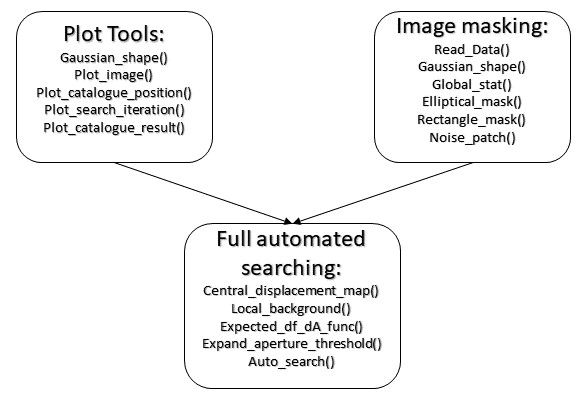
\includegraphics[width=\linewidth]{Figure_9.jpg}
    \caption{Diagrammatic description of the code structure. The plot tools and image masking modules contained functions that were imported into the fully automated searching module that ran functions from them when needed.}
    \label{fig:1}
\end{figure}

\subsection{Evaluating flux distributions and masking}
The choice to evaluate the local noise distributions as opposed to the global noise distribution arose from the wide variations in apparent background noise levels. By selecting a random segment of the sky of size $50$ (in pixel counts) and plotting a histogram of the pixel flux distribution it was seen that it conformed very well with a Gaussian distribution with a long tail and small peaks representing galaxy sources. The local noise distribution could thus be characterised by fitting a Gaussian to the histogram.\newline
 \begin{figure}[H]
    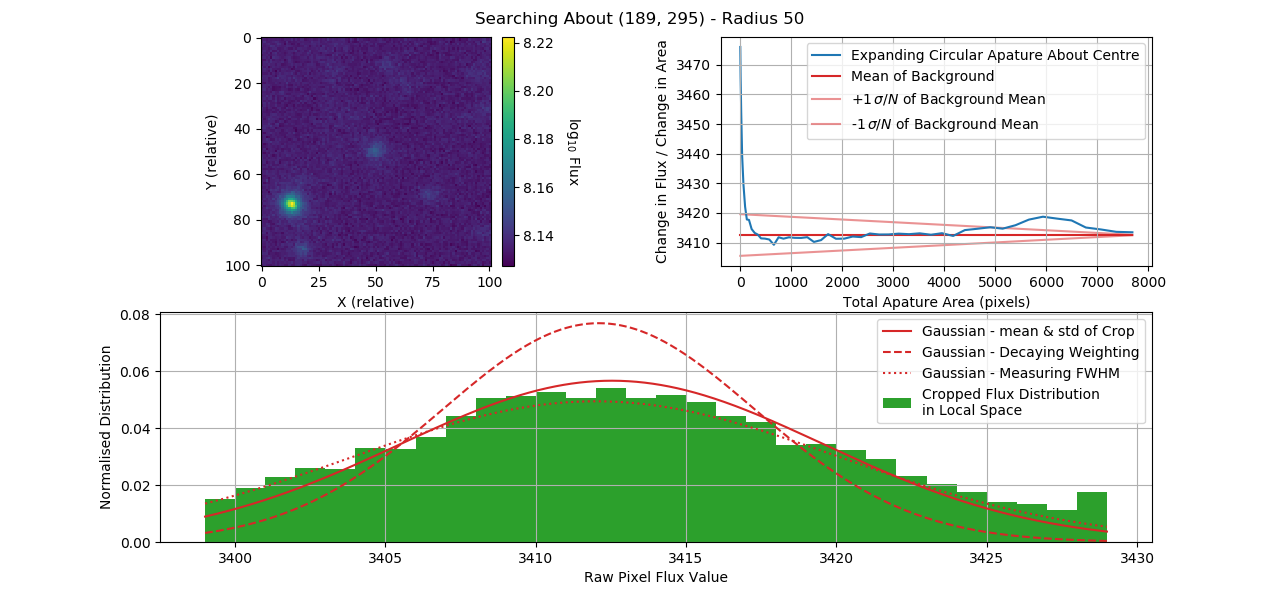
\includegraphics[width = \linewidth]{Figure_4.png}
    \caption{Plot summary of a test galaxy and different types of fits to the flux histogram. The flux histogram contains the galaxy as well and so a pure Gaussian fit will not be effective and correctly characterising the noise distribution. The growth multiplier was set to $1$ for this test.}
    \label{fig:2}
 \end{figure}
 
\noindent It was found that the optimal way of characterising the local noise was to fit the flux distribution by considering its full-width at half maximum (FWHM). This removed flux from the sources in the area being considered. The FWHM was calculated by finding the two pixel flux value bins (bin of integer width to prevent data loss) that corresponded to half of the maximum bin height. Then assuming the noise is distributed as a pure Gaussian function ($\sim\,G(\mu_{noise},\sigma_{noise})$) the FWHM is related to the standard deviation of the assumed noise function through: $FWHM\,=\,2\sqrt{2\sigma^{2}ln(2)}$. It is assumed that the pixel flux bin with the largest height is the noise mean. \newline

\noindent As illustrated in Figure \ref{fig:1}, determining when a galaxy ended was estimated by finding when the change in flux over change in area around a galaxy, $\frac{dF}{dA}\,=\,\frac{\sum_{pixels}F}{Pixels}$, falls within $\pm1\sigma\times STD_growth_multiplier$ of the background noise distribution mean [4]. The growth multiplier enabled different thresholds to be tested. For the background noise, $\frac{dF}{dA}\,\sim\,G(\mu_{noise}, \frac{\sigma_{FWHM}}{\sqrt{N}})$ where $N$ is the number of new pixels being encompassed by the expanding aperture. Note the standard deviations dependence on $N$ [4]. Although the $\pm1\sigma$ choice is arbitrary it was deemed sufficient the signal could be considered noise if it is within $\approx70\%$ confidence range of the background mean (note that the background mean does not have a dependence on $N$).\newline

\noindent An important component of the precision of the galaxy count method is the estimation of the random and systematic errors that contribute to uncertainty on a $log_{10}(N<m)$ - $m$ graph, this is described in the table below.

\begin{center}
 \begin{tabular}{||c c||} 

 \hline
 $log_{10}(N<m)$ error & $m$ error\\ [0.5ex] 
 \hline\hline
 Number count error (\sqrt{N}) & Aperture error \\ 
 \hline
 - & Zero point error  \\
 \hline
 - & Counts above background \\
 \hline
 - & Background removal\\[1ex] 
 \hline

\end{tabular}
\end{center}
The flux count error on each pixel arises from the calculation of the true galaxy flux given by $\delta f = f\,-\,\mu_{noise}$, where $f$ is the flux value of the pixel. Then for each pixel, $\sigma_{\delta f}^{2}\,=\,\sigma_{noise}^{2}\,+\,(\sqrt{\delta f})^2$, where $\delta f$ is the Poisson variance for the average flux count. And $\sigma_{noise}^{2}$ is the background noise variance. For a galaxy we are required to sum over these so the total error contributions for the flux above background and the background removal become $S_{noise}\,=\,\sqrt{A}\sigma_{noise}$ and $S_{\delta} = \sqrt{Galaxy's\, flux}$. Invariably, the thresholding technique will cut-off some flux from the observed galaxy source. Likelihood estimation techniques can therefore be used to use a functional form of a galaxy's flux over area distribution (assumed to be exponential) to calculate a flux cut-off correction and an error associated with it. Generally, $\frac{dF}{dA}\,=\,\beta e^{-\frac{A}{\lambda}}$ with unknown parameters $\beta$ and $\lambda$, these parameters correspond to scaling and decay length and were estimated by fitting an exponential function. By integrating from the cut-off area to $\infty$, an estimate of the amount of flux $\Delta F$ not accounted for by thresholding was found. It follows thus $\Delta F\,=\,\beta\lambda e^{-\frac{A}{\lambda}}$ and $\sigma_{\Delta f}^2\,=\,(\lambda \sigma_{\beta})^2\,+\,(\beta\sigma_{\lambda}(\frac{A}{\lambda}\,+\,1))^2$.\newline

\begin{figure}[H]
    \centering
    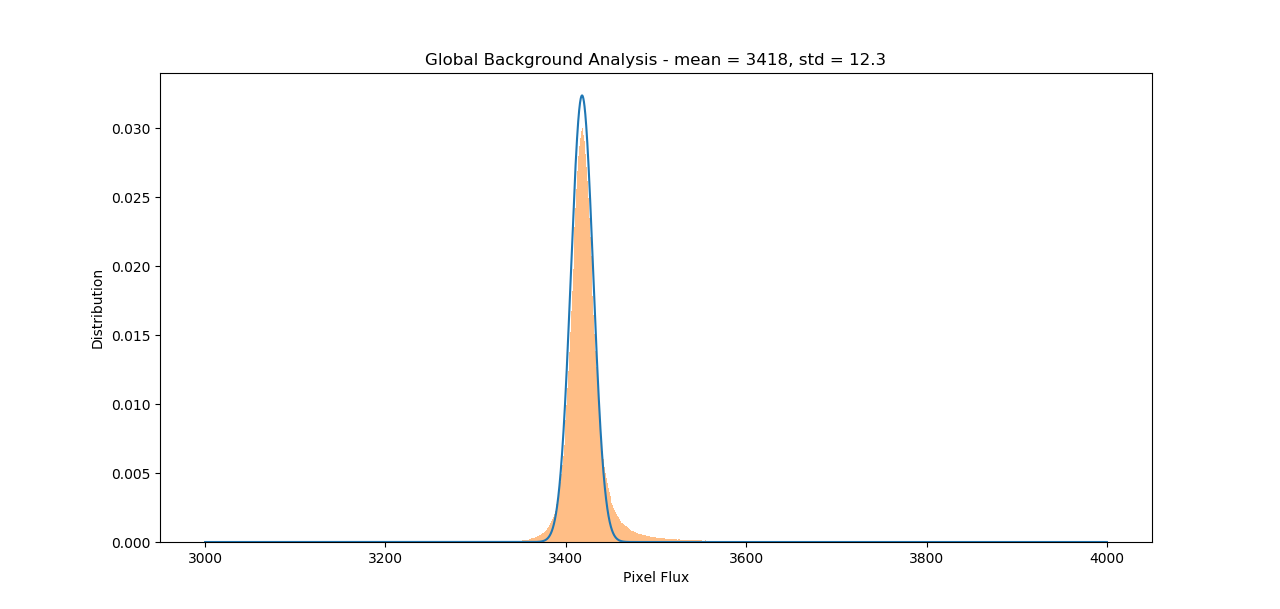
\includegraphics[width = \linewidth]{Figure_5.png}
    \caption{Illustration of global flux histogram and the noise characterisation evaluated through the FWHM technique. Right hand side of distribution clearly shows a tail that arises from the flux of the galaxies, not the background noise.}
    \label{fig:3}
\end{figure}

\noindent Masking of spurious objects on the image was done to remove bloomed pixels from sources that were brighter than the allowed pixel flux of $2^{16}\,=\,65,536$ [1], this will make those sources' fluxes unreliable. To also ensure smooth running of the cataloguing algorithm, the masking needed to be done by filling the spurious objects with random noise. A histogram of the global distribution of fluxes was created and then the FWHM technique used to characterise only the background noise as a Gaussian. Then the \textit{numpy.random} function used to randomly sample flux values to place into spurious pixels. Since the image was represented as 2D array after importing, array splicing was conveniently used to select regions that needed masking.\newline

\begin{figure}[H]
    \centering
    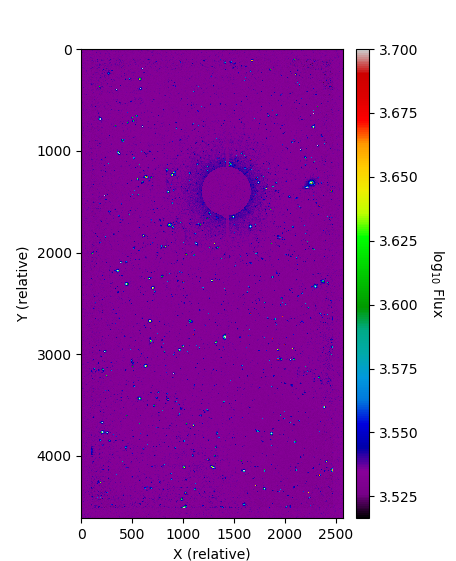
\includegraphics[scale=0.4]{Figure_6.png}
    \caption{CCD image post masking to hide spurious objects. These objects were included bloomed pixels which occur as a result of the pixel's range of intensity detection not being high enough.}
    \label{fig:4}
\end{figure}

\noindent Calibrating flux counts obtained from the CCD to obtain involves comparison with a standard star. Under the AB magnitude system [1] a specific flux density of $3631\,\times\,10^{-26}\,W\,m^{-2}Hz^{-1}$ is defined as zero magnitude, this is the system under which the image was calibrated with. Conversion to flux counts made of use of equation \ref{eq:3} with the addition of the instrument zero point that was included in the image's metadata. In summary, $m\,=\,ZP_{inst}\,-\,2.5log_{10}(flux\_counts)$, where $m$ is the magnitude and $ZP_{inst}$ is the instrument zero point.

\subsection{Automated galaxy finding}
The automatic categorisation algorithm looped over the entire array of pixel flux values and found the maximum, then the aperture expansion algorithm was initiated over those pixel coordinates. To ensure that the algorithm did not continue finding maximum points in noise, a selection multiplier was introduced. This ensured that the maximum pixel flux value was above $1\sigma\times STD\_selection\_multiplier$. The program would stop searching if it was below this limit. This allowed for varying the point at which galaxies stop being detected.\newline

\begin{figure}[H]
    \centering
    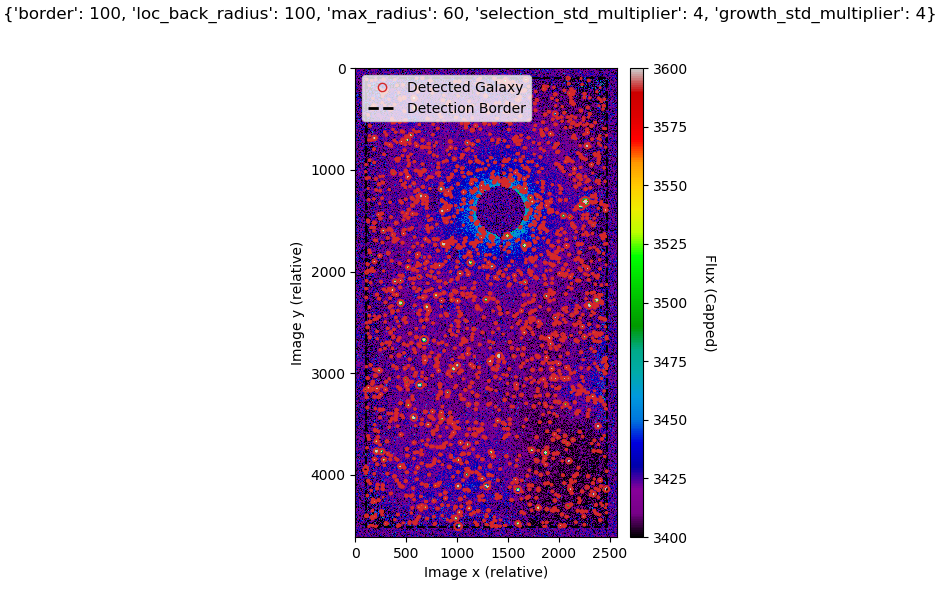
\includegraphics[width = \linewidth]{Figure_7.png}
    \caption{Galaxies detected by the automated categorisation algorithm. The selection multiplier was set to $4\sigma$ and the growth multiplier was set to $4\sigma$. Detected galaxies are encircled with red rings to highlight them as well as for testing purposes.}
    \label{fig:5}
\end{figure}

\noindent Galaxies of radius $1$ pixel (corresponding to a galaxy containing 5 pixels) or less were automatically discarded as it resulted in an enormous number of galaxies and they were considered to be part of the random noise. This meant that very faint galaxies did get removed but this was handled through the error categorisation procedures. \newline

\noindent A consistent error that came up was that apertures on test galaxies sometimes included multiple galaxies. This would skew the source counts. If the gradient of the $\frac{d F}{d A}$ plots increased it meant that another source was likely being detected and so the aperture expansion algorithm was stopped and the area covered set to random noise. Furthermore, the algorithm initially struggled with galaxies of elliptical shape since the aperture area was a circular shape. Generally only two close galaxies were difficult for the algorithm to detect if there were a very large magnitude difference between them.
\begin{figure}[H]
    \centering
    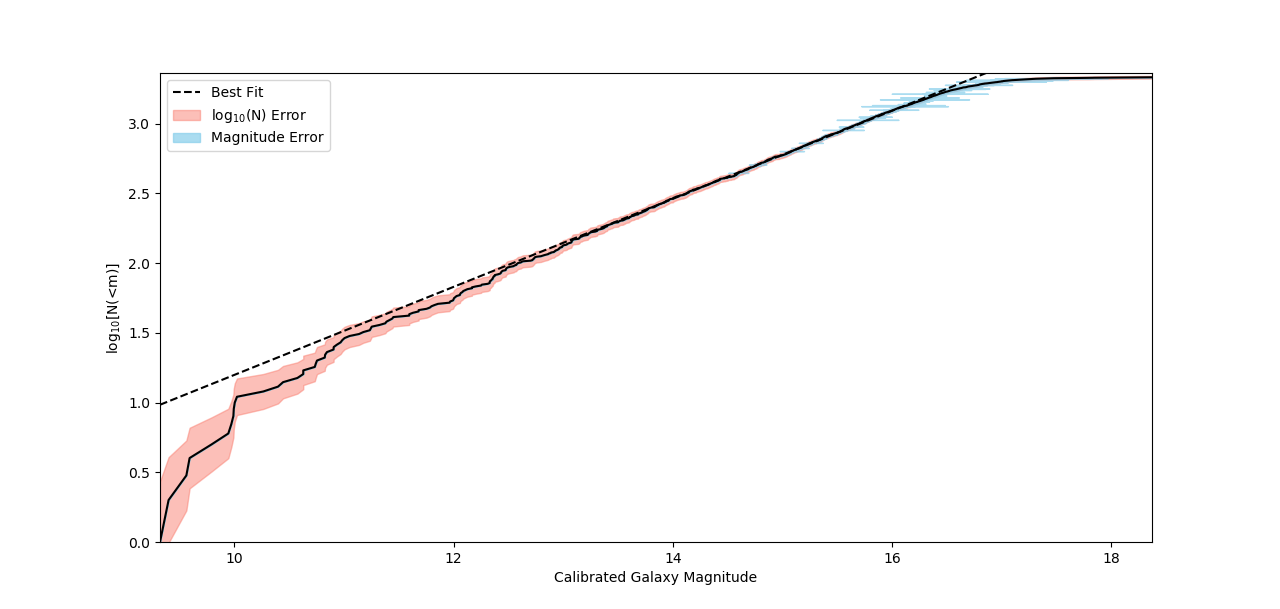
\includegraphics[width = \linewidth]{Figure_8.png}
    \caption{$log_{10}(N(<m))$ against magnitude plot with errors, it was found that due to the dense nature of the galaxy counts areas of the error regions would be shaded. A clear round-off after $m\,=\,16$ as a result of incompleteness [1]. There is also a clear variation from the linear best fit at magnitudes less than $m\,=\,13$ this is attributed to low source counts - brighter galaxies are rarer [1].}
    \label{fig:6}
\end{figure}
\section{Results and analysis}

Figure \ref{fig:6} represents the data for selection multiplier and growth multiplier of $4\sigma$ (away from the background mean), this was a convenient choice since code run-times were not long yet the gradient result yielded did not significantly deviate when the multiplier's were set closer to the background mean. In total, $2181$ galaxies were catalogued across all magnitudes from $m\,=\,0$ to $m\,=\,18$. A gradient of $0.31485101 \pm 2.2283\,\times10^{-4}\, (0.07\%)$ and  intercept of: $-1.94599587 \pm 0.00347798\, (0.18\%)$. This is roughly half of what would have been expected had equation \ref{eq:5} been correct. This data therefore suggests either that the assumptions outlined in the theory section of a Euclidean universe were incorrect, that galactic evolution is indeed a significant factor or that there is significant incompleteness of the source counts. We may derive a dependence on distance by luminosity by breaking assumption (2) and suggesting $L\,\propto\,R^\gamma$. This is an accurate assumption since galactic evolution timescales would be a significant factor in deep field CCD images [3]. The gradient obtained yields a luminosity scaling of $\approx\,L\,\propto\,R^{-1.8}$. Evidently, this indicates that galactic evolution plays a significant role in the luminosity of a galaxy [7], suggesting that the older a galaxy is the less luminous it must be. Which is entirely consistent with the idea that galaxies grow bigger through accretion and must therefore be more luminous through time [8], in addition to the galactic mergers that have been confirmed.\newline

\noindent Introduction to Cosmology by J.V. Narlikar [3] suggests that there is broad agreement amongst many studies that the slope of the $log_{10}N\,-\,m$ curve is significantly flatter than that predicted by equation \ref{eq:5}, corroborating the findings in this investigation. However it suggests the gradient is generally around $\approx\,0.4$ (corresponding to a $\gamma\,\approx\,-1$) not the $\approx\,0.3$ that was found in this study. This still presents a significant difference between this study and others. A solution to this may be found on comparison with Galaxy number counts from the Sloan Digital Sky Survey by Yasuda et al. [2] which suggests that in the magnitude range $16$ to $21$ (in the r band filter which is the same as this investigation) the number counts-magnitude relation is well approximated by equation \ref{eq:5}, however allowing for a amount of galactic evolution [2]. The key difference from this investigation was its use of two independent stripes of the sky (in a magnitude range $12\,\leq\,m\,\leq\,21$) and a sample size of $900, 000$ galaxies. This suggests that this investigation suffered from a low sample size and scope. However, there appears to be very good agreement between figure \ref{fig:6} the general form of the data in Galaxy number counts by Yasuda et al. Specifically, a strong linear trend between magnitudes $12$ and $16$ and a clear flattening up to a magnitude $20$, which arises from incompleteness. The disagreement seems to lie in data for magnitudes less than $12$ which corresponds to brighter galaxies that are fewer in number. The galaxy number counts data seems to suggest a flattening reaching a lower vertical intercept whereas figure \ref{fig:6} illustrates a somewhat erratic behaviour that passes through $0$ on the vertical axis; indicative of a clear deficit in brighter galaxies. Many of the brighter galaxies (or objects) caused bloomed pixels and thus had to be manually masked over; while a large number of very faint but obvious galaxies were missed due to the selection multiplier being too high, thus skewing the number count and potentially leading to a lower than expected gradient. Owing to the large field of view and two independent studies in the galaxy number count investigation it appears that a lack of brighter galaxies has been mitigated. To test this idea another run was taken but this time reducing the selection multiplier to $2\sigma$ from the background mean. This results in a larger galaxy count. If indeed the lack of agreement between this investigation and all other sources is due to a low sample count then a sharp increase in gradient should appear. This test yielded a sample size of $3798$ galaxies, a gradient of: $0.32229380 \pm 1.1213\times10^{-4} \,(0.03\%)$ and intercept of:$-2.05590937 \pm 0.00175312\,(0.09\%)$ for the linear fit - a clear increase in gradient. While this indicates a low sample size effect in figure \ref{fig:6} it is not conclusive evidence. Testing with an even lower selection multiplier could be taken to investigate this further. The low number count at low magnitudes due to masked out objects could have been accounted for by adding in sources. A measure of incompleteness as a function of magnitude would have also aided in identifying low sample sizes. A factor not accounted for in this investigation is the different luminosity classes of different galaxies [9] and the differences in galactic evolution between them as evidenced by distinct jumps in figure \ref{fig:5}.

\section{Conclusion}
This paper presented the number counts of galaxies taken on a deep optical CCD image with an SDSS r band filter over a magnitude range of $9$ to $18$. Primarily this paper detailed the procedures and error analysis of an automated galaxy count of an image, accounting for errors contributing to the number counts and the magnitudes. We compared the data with external sources, notably Galaxy number counts by Yasuda et al. and Introduction to Cosmology by J.V. Narlikar to demonstrate the successes and failings of this study. We see that although there are some strong agreements between these sources and this investigation, they do not corroborate the same gradient for the $log_{10}N\,-\,m$ curve. There is clear evidence that this is attributable to a low sample size effect in this investigation. However, both the external sources and this investigations reject gradient implied by equation \ref{eq:5} due to the assumption of a fixed luminosity for all galaxies being false.
\begin{thebibliography}{1}

\bibitem{c1} Astronomical image processing lab script, R. Oulton

\bibitem{c2} Yasuda 2001

\bibitem{c3}  Introduction to Cosmology, J.V. Narlikar

\bibitem{c4} Statistics of measurement 

\bibitem{c5} https://docs.scipy.org/doc/numpy-1.14.0/reference/routines.random.html

\bibitem{c6} Code on github

\bibitem{c7} http://icc.dur.ac.uk/~tt/Lectures/Galaxies/TeX/lec/node85.html

\bibitem{c8} https://www.nature.com/articles/s41550-018-0436-x.pdf

\bibitem{c9} https://ned.ipac.caltech.edu/level5/CLASSIFICATION/lucl.html

\bibitem{c10} UCI, Millikan oil drop data analysis [Online] Available at: \url{https://www.physics.uci.edu/~advanlab/millikan.pdf}, Feb. 2019

\bibitem{c11} Sim Scale, What is the reynolds number? [Online] Available at: \url{https://www.simscale.com/docs/content/simwiki/numerics/what-is-the-reynolds-number.html}, Feb. 2019

\bibitem{c12} M. Fowler, Brownian motion [Online] Available at: \url{http://galileo.phys.virginia.edu/classes/152.mf1i.spring02/BrownianMotion.htm}, Feb. 2019

\bibitem{c13} M. D. Allen and O. G. Raabe, Re-evaluation of Millikan’s Oil Drop Data for Small Particles in Air, J. Aerosol Sci. 13, 537 (1982)

\bibitem{c14} British Geological Survey, World magnetic model 2015 calculator [Online] Available at: \url{http://www.geomag.bgs.ac.uk/data\_service/models\_compass/wmm\_calc.html}, Feb. 2019

\bibitem{c15} National Institute of Standard and Technology, elementary charge 
 $e$ [Online] Available at: \url{https://physics.nist.gov/cgi-bin/cuu/Value?e|search\_for=charge}, Feb. 2019

\end{thebibliography}


\end{document}

